% siminos/CLE/CLE.tex
% $Author$ $Date$

                            \newif\ifdraft \newif\ifpaper
\drafttrue\paperfalse       % draft version, commented
% \draftfalse\papertrue     % final version, no comments
%%%%%%%%%%%%%%%%%%%%%%%%%%%%%%%%%%%%%%%%%%%%%%%%%%%%%%%%

% Predrag reorganized siminos/CLE/          2009-10-09
% Vaggelis created siminos/CLE/CLE.tex      2009-09-21
% Vaggelis created siminos/CLE              2009-02-05

\documentclass[aps,pre,preprint,groupedaddress]{revtex4}
%\documentclass[aps,prl,preprint,superscriptaddress]{revtex4}
%\documentclass[aps,prl,twocolumn,groupedaddress]{revtex4}

\bibliographystyle{apsrev}
\usepackage{amsmath,amsfonts,amssymb,amsbsy,amscd}
\usepackage{ifthen}
\usepackage[dvips]{graphicx}
\usepackage[dvips]{color}
\usepackage[dvips,colorlinks]{hyperref}

\input ../inputs/def
%\input ../inputs/defsThesis.tex
\input inputs/defsCLE.tex

\begin{document}
% \title{Towards continuous symmetry reduction in high dimensional flows}
\title{Returm maps of high dimensional flows with continuous symmetry I: symmetry reduction}
\author{Evangelos Siminos}\email[]{siminos@gatech.edu}
\author{Predrag Cvitanovi\'c}
%\homepage[]{Your web page}
%\thanks{}
%\altaffiliation{}
\affiliation{Center for Nonlinear Science,
School of Physics, Georgia Institute of Technology,
Atlanta, GA 30332-0430}

\date{\today}

\begin{abstract}
% insert abstract here
\end{abstract}

% insert suggested PACS numbers in braces on next line
\pacs{}
% insert suggested keywords - APS authors don't need to do this
%\keywords{}

\maketitle

\section{\label{s:intro} Introduction}
% Put \label in argument of \section for cross-referencing
%\section{\label{}}
    \input intro

\subsection{\label{s:introCLE} \CLe}
    % siminos/CLE/introCLE.tex
% $Author$ $Date$

% introducing CLe
% from siminos/thesis/lasersSym.tex

\CLe\ (henceforth CLE) were introduced by Gibbon and McGuinness\rf{GibMcCLE82} as a low-dimensional model
of baroclinic instability in the atmosphere.
As the name suggests they turned out to be a complex generalization
of Lorenz equations\rf{lorenz}:
\beq
\index{Complex Lorenz equations}
\begin{split}
 \dot{x} &=-\sigma x+ \sigma y \cont
 \dot{y} &=(\rLor-z)x-a y \cont
 \dot{z} &= \frac{1}{2}\left(x y^*+x^*y\right)-b z\,,
 \label{eq:CLe}
\end{split}
\eeq
where $x,y$ are complex variables, $z$ is real, while the
parameters $\sigma,\,b$ are real and $\rLor=\RerCLor+i
\ImrCLor$, $a=1-i e$ are complex.

It can easily be checked that \cLe\ are 
equivariant under the one parameter rotation
group $\Un{1}\cong\SOn{2}$ acting by
\beq\label{eq:SO2cle}
	(x,\,y,\,z)\mapsto (e^{i\theta}x,\,e^{i\theta}y,\,z)\,,\ \theta\in[0,2\pi]\,,
\eeq

Ning and Haken\rf{NingHakenCLE90} have shown
that equations isomorphic to \cLe\ also appear as a
truncation of Maxwell-Bloch equations describing a single
mode, detuned, ring laser.
%with $x,y$ and $z$
%proportional to electric field, polarization and population inversion, respectively.
They set $e+\ImrCLor=0$ so that a detuned
\eqv\ exists.
    \ES{This assumption is questionable unless it
is forced by the physics of the problem, which I cannot
follow very well. It leads to non-generic bifurcation
behavior, while one would like a model of a physical system
to be robust under perturbations (of the model). Furthermore,
the fact that the Hopf cycle in the general case is an
$\SOn{2}$-orbit has gone unnoticed. The \reqv\ can be
interpreted as an \eqv\ in a rotating frame and the measured
electric field of the laser would be the same in both cases.
    }
In contrast Bakasov and Abraham\rf{BakasovAbraham93} only require
that a \emph{relative equilibrium}, see \refsect{s:symDyn}, exists
and show that one can use
\CLe\ with $\ImrCLor=0$ and $e \neq 0$ to describe detuned lasers.
Here we follow the choice of Bakasov and Abraham, since as shown by Krupa\rf{Krupa90} 
it corresponds to the generic bifurcation senario in a system with the symmetry
of CLE. Moreover, in all numerical examples
that follow, the parameters will be set to the Lorenz values
$\RerCLor=28,\, b=8/3,\, \sigma=10$, with the ``detuning'' $e=1/10$ unless explicitly
stated otherwise. Note that $e$, although related to detuning in Maxwell-Bloch equations
is not directly proportional to it\rf{BakasovAbraham93}.

\PublicPrivate{}{
 \refFig{fig:CLE} illustrates the need
 to project dynamics on \reducedsp: Dynamics is organized by
 the interplay of the stable and unstable manifolds of \eqv\
 \EQV{0} and \reqv\ \REQV{}{1} but the dynamics along the
 direction of rotation blur the picture and the notion of
 recurrence becomes relative. We will present various
 approaches to orbit space reduction in the following.
% sections.
    }

    \ES{move to elsewhere: ``
The lowest level of organization of the
familiar (real) Lorenz system that does not posses a
continuous symmetry can be
understood\rf{DasBuch,SiminosThesis} in terms of the unstable
manifolds of the equilibrium at the origin and the two
(discrete-symmetry-related) equilibria $\EQV{1,2}$. In the
case of {\cLe}  the origin \EQV{0} is an \eqv\ of
\refeq{eq:CLe} for any value of the parameters. As shown in
\refref{FowlerCLE82} it is stable for $0<\RerCLor<\rho_{1c}$
and unstable for $\rho_{1c}<\RerCLor$, where
\beq
	\rho_{1c} = 1 + \frac{(e+\ImrCLor)(e-\sigma \ImrCLor)}{(\sigma+1)^2}\,.
\eeq
At bifurcation a pair of eigenvalues crosses the imaginary axis with imaginary part:
\beq
	\omega_c = \frac{\sigma (e + \ImrCLor)}{\sigma+1}\,.
	\label{eq:omegaCLE}
\eeq
and a \emph{relative equilibrium} \REQV{}{1}, an equilibrium
in a frame rotating with constant angular velocity is born.
Alternatively we might say that a relative equilibrium is a
periodic orbit that is invariant (as a set) under the action
of $\LGelement{l_p}\in\Group$ for any $l_p$.
    \ES{this implies constant angular velocity by
    equivariance.}
    \ES{Does not fit here, but keep: For $e+\ImrCLor=0$ the
    relative equilibrium degenerates to an \SOn{2}-orbit of
    \eqva\rf{FowlerCLE82}, since $\omega_c =0$.}
As we will see in \refsect{s:StabReq}, \REQV{}{1} of {\cLe}
for the parameter set we study here is unstable with one
complex expanding eigenvalue. Yet, being a periodic orbit,
its unstable manifold is three-dimensional, with one
eigendirection corresponding to the direction of $\vf$ which
also coincides with the direction of rotations of the system.
In \reffig{fig:CLE} we plot one trajectory on the unstable
manifold of \REQV{}{1}. While it spirals away from
$\REQV{}{1}$ it also ``drifts'' along the direction of
rotations of the system. This drifting motion obscures
understanding of the stretching mechanism along the expanding
eigendirection and subsequently the folding of the unstable
manifold back to itself.
    ''} %end \ES{move to elsewhere: ``
%
%%%%%%%%%%%%%%%%%%%%%%%%%%%%%%%%%%%%%%%%%%%%%%%%%%%%%%%%%%%%
\begin{figure}[ht]
\begin{center}
  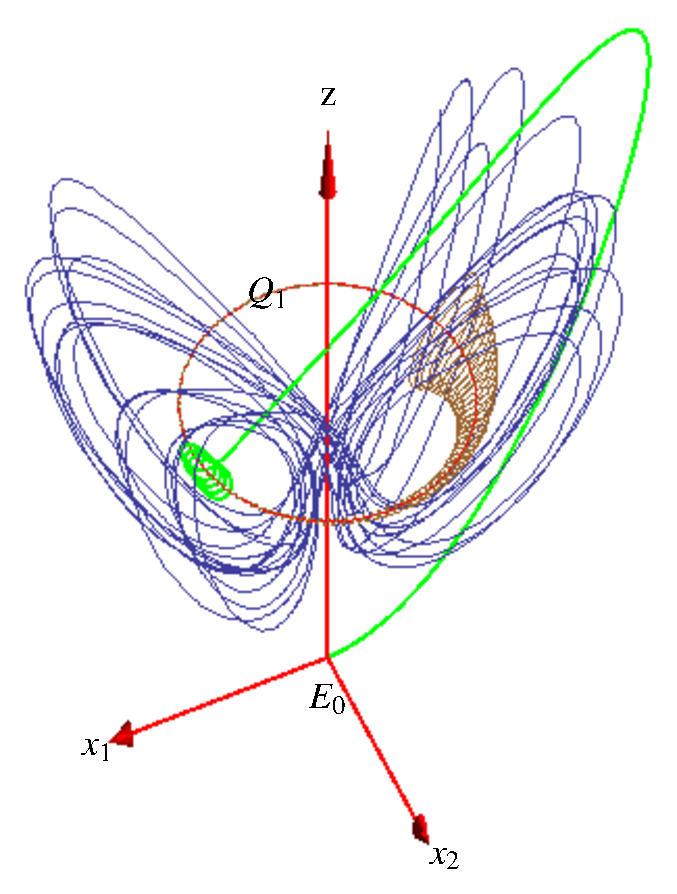
\includegraphics[height=0.25\textheight]{../figs/CLE}
\end{center}
\caption[Complex Lorenz flow phase space]
{ \Statesp\ portrait of \cLe\ dynamics for $e=1/10,\,
\ImrCLor=0$. Plotted are \reqv\ \REQV{}{1} (red), its unstable
manifold (brown), \eqv\ \EQV{0}, a representative of its
unstable manifold (green), 3 repetitions of \rpo\
``01''(magenta) and a generic orbit (blue).}
\label{fig:CLE}
\end{figure}
%%%%%%%%%%%%%%%%%%%%%%%%%%%%%%%%%%%%%%%%%%%%%%%%%%%%%%%%%%%%
%


\ES{move elsewere: The next (or a complimentary) level of organization of (real)
{\Le} attractor is provided by the dense set of \po s
embedded in it\rf{DV03,DasBuch}. In {\cLe} a secondary
bifurcation from \REQV{}{1} is expected, according to Krupa's
theorem\rf{Krupa90}, to result in \emph{relative periodic
orbits} that satisfy
\beq
	\LGelement{l_p}x(t+T_p)=x(t)\,,
\eeq
{\ie} they ``return'' after a time period $T_p$ to a point
that maps to the initial one under a group transformation
$\LGelement{l_p}$ with group parameter period $l_p$. A {\rpo}
of {\cLe} is shown in \reffig{fig:CLE} as its iterations fill
a torus. Therefore we see that in systems with continuous
symmetry we have to account for tori instead of {\po s} as
the organizational blocks of the attractor.
}



\subsection{\CLe\ \reqva}

To find the location of the \reqv\ it is convenient to work
on polar coordinates defined by $x=r_1 e^{i \phi_1},\,y=r_2
e^{i \phi_2}$. Equations \refeq{eq:CLe} take the form
    %PC: Rebecca and I rederived these: they check.
\beq
\begin{split}
	\dot{r}_1 &=-\sigma (r_1 - r_2\cos\phi) \cont
	\dot{r}_2 &=-r_2 + r_1(\RerCLor -z)(\cos\phi-\ImrCLor\sin\phi) \cont
	\dot{z} &=  -b z+r_1 r_2\cos\phi \cont	
	\dot{\phi} &=-e-\frac{\sigma r_2 \sin\phi}{r_1}-\frac{r_1(\RerCLor-z) (\ImrCLor\cos\phi+\sin\phi) }{r_2}\,,
	\label{eq:CLePolar}
\end{split}
\eeq
where $\phi=\phi_1-\phi_2$ and the evolution equations for
$\phi_1,\phi_2$ are given by
\beq
\begin{split}
	\dot{\phi}_1 &=-\frac{\sigma r_2 \sin\phi}{r_1}\cont
	\dot{\phi_2} &= e +\frac{r_1\left( (\RerCLor -z)\sin\phi+\ImrCLor\cos\phi\right)}{r_2}\,.
	\label{eq:CLeAngl}
\end{split}
\eeq

For simplicity we now turn to the ``laser case''
$e\neq0,\;\ImrCLor=0$; in the numerical examples we set the
detuning to $e=1/10$.

The condition for a \reqv~ is that all time derivatives in
\refeq{eq:CLePolar} vanish from which we get
% Explicit form here, simplified in terms of z component below
% \beq
% \begin{split}
% 	z &= -\frac{e^2}{(\sigma +1)^2}+\RerCLor -1\cont
% 	r_2 &= \frac{\sqrt{-b \left(e^2+(\sigma +1)^2\right)\left(e^2-(\RerCLor -1) (\sigma +1)^2\right)}}{(\sigma+1)^2}\cont
% 	r_1 &= \frac{\sqrt{-b \left(e^2-(\RerCLor -1) (\sigma +1)^2\right)}}{\sigma +1}\cont
% 	\Phi &= -\cos ^{-1}\left(\frac{\sigma +1}{\sqrt{e^2+(\sigma +1)^2}}\right)
% \end{split}
% \eeq
\beq
\begin{split}
	z^{(1)} &= \frac{-e^2+(\RerCLor -1)(\sigma +1)^2}{(\sigma +1)^2}\cont
	r_1^{(1)} &= \sqrt{b z^{(1)}}\cont
	r_2^{(1)} &= \sqrt{b \left(e^2+(\sigma +1)^2\right)z^{(1)}}\cont
	\phi^{(1)} &= -\cos ^{-1}\left(\frac{\sigma +1}{\sqrt{e^2+(\sigma +1)^2}}\right)
\end{split}
\eeq
Substituting in \refeq{eq:CLeAngl} we get $\dot{\phi}_1=\dot{\phi}_2=e \sigma/(1 + \sigma)\neq 0$ for $e\neq0$
and thus we have indeed a \reqv, not a group orbit of \eqva.

Calculation  in polar coordinates $r_1,r_2,\phi,z$ of stability eigenvalues for \REQV{}{1}
for the set of parameters we use here yields
\beq
	\eigRe[1]\pm i\eigIm[1]= 0.0938\pm 10.1945i,\,
    \eigExp[3]=-11.0009,\, \eigExp[4]= -13.8534\,.
	\label{eq:CLeREQBstab}
\eeq


\section{\label{s:symDyn} Symmetry of dynamical systems}
    \input symDyn

\section{\label{s:symRedGeneral} Symmetry reduction methods}
    \ES{Move moving frames to each own section}
    \input symRedGeneral
    \input Hilbert
    \input movingFrames
    \input slice
    \input mfLocal

\section{Stability of \reqva}
    \input stabReqva

% Specify following sections are appendices. Use \appendix* if there
% only one appendix.
%\appendix
%\section{}

% If you have acknowledgments, this puts in the proper section head.
%\begin{acknowledgments}
% put your acknowledgments here.
%\end{acknowledgments}

% Create the reference section using BibTeX:
\bibliography{../bibtex/siminos}

\end{document}
